\chapter{Context}
앱을 개발하다보면 항상 Context 클래스를 만나게 된다. 
Context가 없으면 Activity를 시작할 수도, Broadcast를 발생시킬 수도, Service를 실행할 수도 없다. 
리소스에 접근할 때도 Context를 통해야만 가능하다.
Context는 여러 컴포넌트의 상위 클래스면서 Context를 통해서 여러 컴포넌트가 연결돼 있으므로   Context 자체에 대해서 살펴보는 것은 컴포넌트를 이해하는 데도 도움이 된다.\\

Context는 추상 클래스인데 메서드 구현이 거의 없고 상수 정의와 추상 메서드로 이루어진다. 
그럼 Context의 하위 클래스는 어떤 게 있는가? 주요한 것을 얘기하면, 직접 상속한 것은 ContextWrapper이고 ContextWrapper를 상속한 Activity, Service, Application이 있다(BroadcastReceiver, ContentProvider는 Context를 상속한 것이 아니다).\\

% http://blog.naver.com/PostView.nhn?blogId=huewu&logNo=110085457720&parentCategoryNo=&categoryNo=&viewDate=&isShowPopularPosts=false&from=postView
Context와 컴포넌트 중간에 있는 ContextWrapper를 먼저 살펴보자.
ContextWrapper 클래스는 그 이름처럼 Context를 래핑한 ContextWrapper(Context base) 생성자를 갖고 있다.
\begin{lstlisting}[frame=single, caption=ContextWrapper.java]
    Context mBase;

    public ContextWrapper(Context base) { // (1)
        mBase = base;
    }

	protected void attachBaseContext(Context base) { // (2)
        if (mBase != null) {
            throw new IllegalStateException("Base context already set");
        }
        mBase = base;
    }
    
    public Context getBaseContext() {
        return mBase;
    }
    
    ...
    
    @Override
    public Context getApplicationContext() {
        return mBase.getApplicationContext(); // (3)
    }
    
    ...
    
    @Override
    public void startActivity(Intent intent, Bundle options) {
        mBase.startActivity(intent, options); // (4)
    }
    
    ...
    
    @Override
    public void sendBroadcast(Intent intent) {
        mBase.sendBroadcast(intent); // (5)
    }

	... 
	
    @Override
    public Resources getResources() {
        return mBase.getResources(); // (6)
    }
\end{lstlisting}
\begin{itemize}
\item 3라인(1), 7라인(2)에서 base 파라미터에 전달되는 것은 Context의 여러 메서드를 직접 구현한 ContextImpl 인스턴스이다. 
ContextImpl은 앱에서 생성해서 사용할 수 있는 public 클래스는 아니지만, 소스는 공개되어 있으니 한번씩은 살펴보도록 하자.

\item ContextWrapper의 여러 메서드는 base의 메서드를 그대로 다시 호출하고 있다(3, 4, 5, 6).

\item Activity, Service, Application은 3라인(1)의 생성자를 사용하지 않고, 실제로는 7라인(2)의 attachBaseContext()를 사용한다. Activity, Service, Application 모두 내부적으로 ActivityThread에서 컴포넌트를 시작하면서 내부적으로 각 컴포넌트의 attach() 메서드를 실행하고 attach() 메서드에서 또다시 attachBaseContext()를 실행하는 것을 볼 수 있다.
\end{itemize}

이제 또 다른 질문을 해보자. 그럼 ContextImpl은 앱에서 싱글톤으로 단 하나의 인스턴스를 가지고서 ContextWrapper에 전달하는가?
이것은 ContextWrapper에 getBaseContext()와 getApplicationContext()라는 2개의 메서드가 별도인 것을 보면 싱글톤이 아닌 것을 유추할 수 있다.\footnote{Context에는 getBaseContext() 메서드는 없고 getApplicationContext() 메서드만 있다.}\\

Activity, Service, Application 컴포넌트는 각각 생성한 ContextImpl을 하나씩 Wrapping하고 있고 getBaseContext()는 각각 ContextImpl 인스턴스를 리턴한다. getApplicationContext()는 Application 인스턴스를 리턴하는 것으로 Application은 앱에서 1개 밖에 없고 어디서나 동일한 인스턴스를 반환한다.\\

ContextImpl을 보면 3가지 정도로 메서드 범주를 나눌 수 있다.
\begin{itemize}
\item 앱 패키지 정보, 내/외부 파일, SharedPreferences, 데이터베이스 등과 관련한 Helper 메서드가 있다. 

\item Activity, BroadcastReceiver, Service와 같은 컴포넌트 관련 메서드와 퍼미션 체크 메서드가 있고, 이들 메서드는 system\_server 프로세스의 ActivityManagerService의 메서드를 다시 호출한다. 

\item ActivityManagerService 를 포함한 시스템 서비스에 접근하기 위해서 getSystemService() 메서드가 있다. 
ContextImpl의 정적 초기화 블록(static initializer block)에서 클래스가 최초 로딩될 때 시스템 서비스를 매핑하고, 이후에는 getSystemService() 메서드에서 매핑을 바로 사용하고 있다.
% http://warmz.tistory.com/50에서 초기화 블록 내용을 알아보자.
시스템 서비스는 Context 클래스에서 XXX\_SERVICE와 같이 상수명으로 모두 매핑되어 있고, Context가 전달되는 어디서든 getSystemService(Context.ALARM\_SERVICE)와 같이 시스템 서비스를 가져다 쓸 수 있다.
\end{itemize}

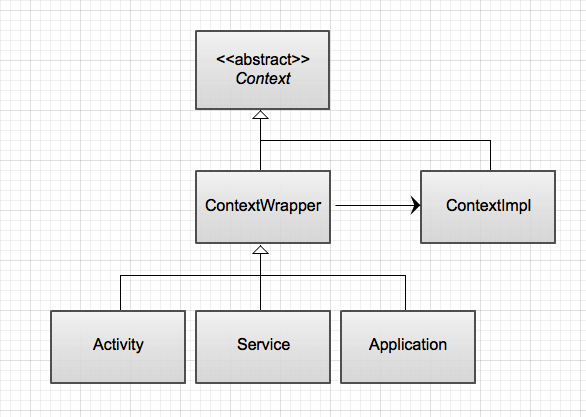
\includegraphics[scale=0.5]{context}\\
객체지향의 원칙에서 상속보다는 구성을 사용하라고 하는데, 이 클래스 다이어그램을 보면 원칙에 들어맞는다.
바로 Activity, Service, Application에서 ContextImpl을 직접 상속하지 않고, ContextImpl의 메서드를 호출하는 형태이다. 이렇게 하면 ContextImpl의 변수가 노출되지 않고, ContextWrapper에서는 ContextImpl의 public 메서드만 호출하게 된다. 또한 각 컴포넌트별로 사용하는 기능에 대한 제어도 단순해진다.\\
%ContextWrapper 소스에 있는 내용

코드에서 Context를 쓰는 방법을 생각해보자.
Activity를 예로 들어보면 여기서 쓸 수 있는 Context 인스턴스는 3개가 된다. 
\begin{enumerate}
\item Activity 인스턴스 자신(this)
\item getBaseContext()를 통해 가져오는 ContexImpl 인스턴스
\item getApplicationContext()를 통해 가져오는 Application 인스턴스: Activity의 getApplication() 메서드로 가져오는 것과 같은 인스턴스이다.
\end{enumerate}

각각의 인스턴스가 다르므로 캐스팅을 함부로 하면 안된다. 이를테면 getBaseContext()로 가져온 것을 Activity로 캐스팅하면 ClassCastException이 발생한다.\\

View 클래스를 보면 생성자에 Context가 들어간다. 이 Context가 어디서 온 것인지 아래 코드를 통해 확인해보자.
\begin{lstlisting}[frame=single]
    @Override
    public void onCreate(Bundle savedInstanceState) {
        super.onCreate(savedInstanceState);
        setContentView(R.layout.main);
        statusView = (TextView) findViewById(R.id.status_view);
        Log.d("suribada", (statusView.getContext() == this));
        Log.d("suribada", (statusView.getContext() == getBaseContext()));
        Log.d("suribada", (statusView.getContext() == getApplicationContext()));
    }
\end{lstlisting}
첫 번째 로그에서만 true가 나오는 것을 볼 수 있다. View 클래스는 생성자에 Context가 전달되어야 한다. 테스트해보면 Activity에서 쓸 수 있는 3가지 Context 모두 다 전달 가능하다. 그러나 View와 연관이 깊은 것은 Activity이므로 Activity를 전달하는 것을 이해할 수 있을 것이다.
내부적으로 setContentView() 메서드에서 사용하는 LayoutInflator에 Activity 인스턴스가 전달되고, View 생성자의 Context 파라미터에 Activity 인스턴스가 전달된다. 
